In questo esempio verrà eseguito il sistema su di un'unica macchina
sfruttando l'interfaccia di loopback.
Per eseguire il server aprire il terminale nella cartella \emph{server}
creata durante l'installazione ed eseguire il comando:\\
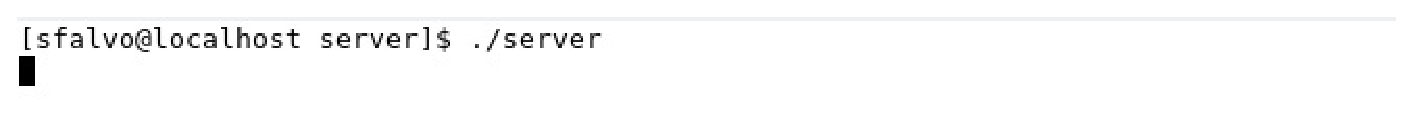
\includegraphics[scale=0.5]{images/esempio/srv_launch}\\
In questo modo viene lanciato il server con i seguenti parametri di default:
\begin{itemize}
\item[T]: 500 
\item[P]: 20
\item[N]: 50
\item[adaptive]: 0 (false)
\item[port]: 5193 
\end{itemize}
Lato client, aprire il terminale nella relativa cartella, ed eseguire il 
comando\\ 
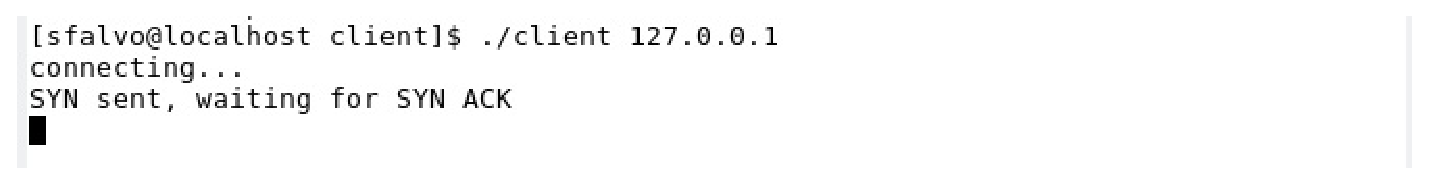
\includegraphics[scale=0.5]{images/esempio/cli_connect}\\
Verra eseguito il client che tenterà ripetutamente di
connettersi al server.\\
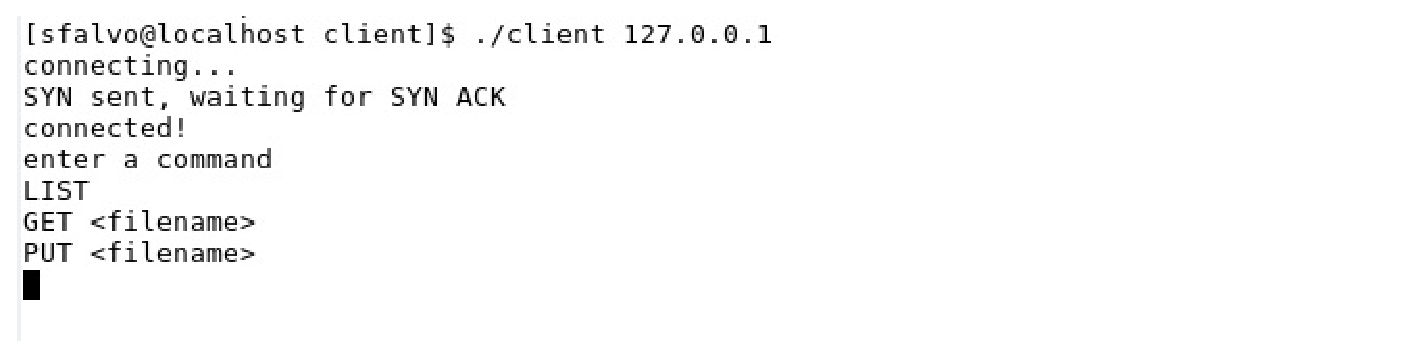
\includegraphics[scale=0.5]{images/esempio/cli_wait}\\
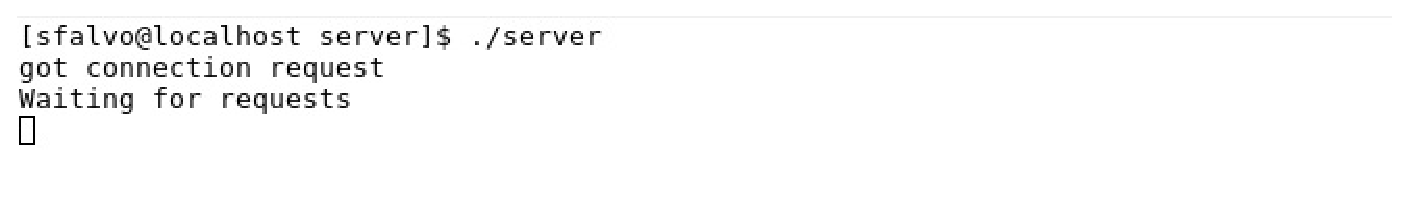
\includegraphics[scale=0.5]{images/esempio/srv_wait}\\
Una volta connessi, inserire uno dei comandi suggeriti, ad esempio il comando LIST\\
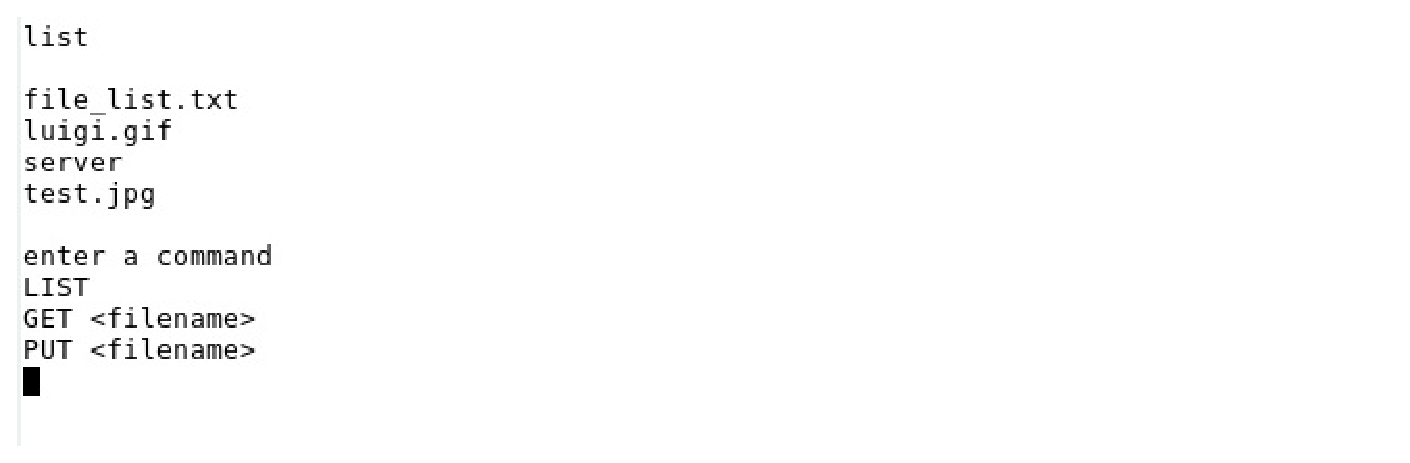
\includegraphics[scale=0.5]{images/esempio/cli_list}\\
Ed ora si può procedere a scaricare uno dei file presenti sul server
tramite il comando GET:\\

\includegraphics[scale=0.5]{images/esempio/cli_get}\\
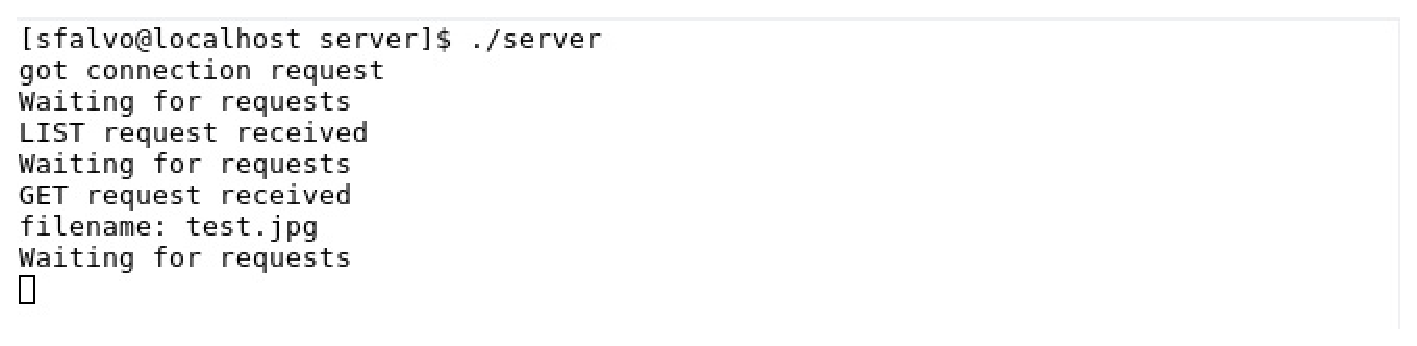
\includegraphics[scale=0.5]{images/esempio/srv_resp}\\
Successivamente si può verificare la presenza del file tramite il comando ls.\\
Per eseguire il server con parametri personalizzati specificare le opzioni
come argomenti del programma, ad esempio:\\
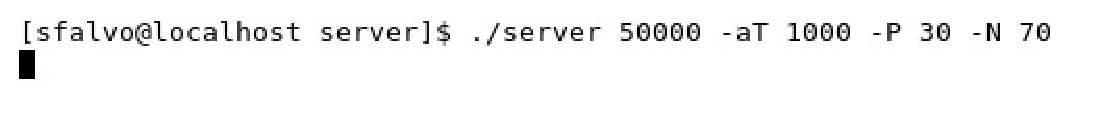
\includegraphics[scale=0.5]{images/esempio/srv_par}\\
In questo modo viene lanciato il server con i seguenti parametri:
\begin{itemize}
\item[T]: 1000
\item[P]: 30
\item[N]: 70
\item[adaptive]: 1 (false)
\item[port]: 5193 
\end{itemize}
Opzioni server:
\begin{itemize}
\item[T]: valore del timeout in millisecondi
\item[P]: probabilità di perdita in percentuale
\item[N]: ampiezza della finestra del protocollo rdt
\item[a]: il protocollo deve avere timeout adattativo
\item[port]: porta di ascolto del server
\end{itemize}
Tutte le opzioni vanno immesse con il trattino che le precede e il valore che le segue.
